% Thesis chapter, plain-language version. Standalone-compilable; to drop into a thesis,
% keep the body and discard the preamble.
%
% Every number comes from paper/thesis_numbers.tex and paper/thesis_count_table.tex, and
% every figure from figures/thesis_fig*.png. All are written by
%   python experiments/thesis_figures.py
% from the run pickles. Nothing below is transcribed by hand.

\documentclass[11pt]{report}
\usepackage[margin=1.1in]{geometry}
\usepackage{amsmath,amssymb,booktabs,graphicx,microtype}
\usepackage[T1]{fontenc}
\usepackage[font=small,labelfont=bf]{caption}
\usepackage{hyperref}
\hypersetup{colorlinks=true,allcolors=blue!55!black}
\graphicspath{{../figures/}}

% generated by experiments/thesis_figures.py, do not edit
\newcommand{\thLossOne}{0.755}
\newcommand{\thLossTwo}{0.503}
\newcommand{\thLossFour}{2 \times 10^{-5}}
\newcommand{\thTriv}{1.007}
\newcommand{\thPredOne}{0.756}
\newcommand{\thPredTwo}{0.504}
\newcommand{\thStairMaxErr}{0.030}
\newcommand{\thStairRuns}{6}
\newcommand{\thMixMin}{0.27}
\newcommand{\thMixOnTarget}{0.98}
\newcommand{\thMixRank}{4}
\newcommand{\thDenseFourLoss}{2 \times 10^{-5}}
\newcommand{\thFinalShare}{6.4}
\newcommand{\thFinalOn}{5}
\newcommand{\thThrSlope}{0.29}
\newcommand{\thThrErr}{1.53}
\newcommand{\thThrMatch}{17/17}
\newcommand{\thLoopErr}{0.00}
\newcommand{\thLoopBad}{11/49}
\newcommand{\thGateBad}{13/50}
\newcommand{\thPruneErr}{0.13}
\newcommand{\thPruneBad}{0/15}
\newcommand{\thLocalErr}{0.83}
\newcommand{\thLocalBad}{0/6}
\newcommand{\thLocalTwo}{4}
\newcommand{\thLocalCompute}{0.39}
\newcommand{\thGateCompute}{0.42}
\newcommand{\thPruneCompute}{0.43}
\newcommand{\thTargetPlain}{2.07}
\newcommand{\thTargetGate}{0.28}
\newcommand{\thSlowErr}{5.17}
\newcommand{\thEpsErrMax}{0.00}
\newcommand{\thWorstGate}{16.7}
\newcommand{\thWorstPrune}{26.0}
\newcommand{\thWorstLocal}{0.5}
\newcommand{\thBelowSame}{5/6}
\newcommand{\thBelowFull}{2/6}
\newcommand{\thRhoDemand}{+0.39}
\newcommand{\thRhoQnorm}{+0.56}
\newcommand{\thRhoEntropy}{+0.56}
\newcommand{\thQsaBad}{20/20}
\newcommand{\thNRuns}{497}


\newcommand{\kstar}{k^\star}
\newcommand{\Ltriv}{L_{\mathrm{triv}}}

\begin{document}
\chapter{How many attention heads does a task need?}

\section{The question}

An attention layer with $H$ heads is hard to read because there are so many heads to
check. At $H = 32$ there are 496 pairs of heads, and far more groups. The usual first step
in interpreting a model is to shrink it: find a small set of heads that does the work, and
study that set instead.

The standard way to shrink a layer is pruning. Each head gets an importance score, and
the $k$ highest-scoring heads are kept \cite{michel2019,voita2019}. Pruning answers the
question \emph{which} heads, but the analyst has to choose \emph{how many}. For
interpretability the number is the interesting part: it is the size of the circuit the
task needs.

This chapter asks whether a model can find that number by itself, during a single training
run. The idea is borrowed loosely from how blood reaches the brain. The total supply is
fixed, so feeding one region means taking from another, and supply follows need. Here
each head receives a share of a fixed total, and a rule decides who gets fed. The biology
is used only as a source of design ideas; nothing in this chapter is a claim about the
brain.

To test any such rule you need a task where the right number of heads is known in
advance. Section~\ref{sec:task} builds one, and explains with simple matrix algebra why it
needs exactly $R$ heads. Section~\ref{sec:supply} defines the supply. Section~\ref{sec:rules}
describes five rules for choosing which heads to feed. Section~\ref{sec:results} gives the
results and Section~\ref{sec:claims} states what they do and do not show.

\paragraph{The findings in one list.}
\begin{enumerate}
\item The task needs exactly $R$ heads. This follows from a rank argument and is confirmed
      by training models of every size.
\item Switching a head's supply to zero removes it exactly. The fed heads form an
      ordinary smaller layer, with no approximation.
\item The obvious rule, ``feed the heads that stand out'', cannot count heads. Its count is
      set by the shape of the demand distribution, not by the task.
\item Rules that compare the loss with a target do find the right count at every task
      size. A standard pruning baseline with the same target does too, so the count
      itself is not something the supply idea uniquely provides.
\item A local rule, where each head must earn its share, removes heads without ever
      letting the model fall back above the ``solved'' bar, and uses about
      \thLocalCompute{} of the compute of a full dense training run.
\end{enumerate}

%=========================================================================================
\section{A task where the answer is known}
\label{sec:task}

\subsection{The task in words}

The model reads a memory of $N = 16$ slots. Each slot $j$ holds two things: a code for its
position, and a random content vector $c_j \in \mathbb{R}^m$. A query token carries a
position $p$. The model must return the contents stored at $R$ fixed offsets from $p$:
\begin{equation}
  \text{target} \;=\; \bigl(\, c_{p+\delta_1},\; c_{p+\delta_2},\; \dots,\; c_{p+\delta_R} \,\bigr),
  \label{eq:target}
\end{equation}
with positions counted modulo $N$. The offsets are spread evenly; with $N = 16$ and $R = 4$
they are $\delta = (1, 5, 9, 13)$. Figure~\ref{fig:task}a shows one query. It carries
$p = 8$ and must return the contents of slots $9, 13, 1$ and $5$.

\begin{figure}[t]
  \centering
  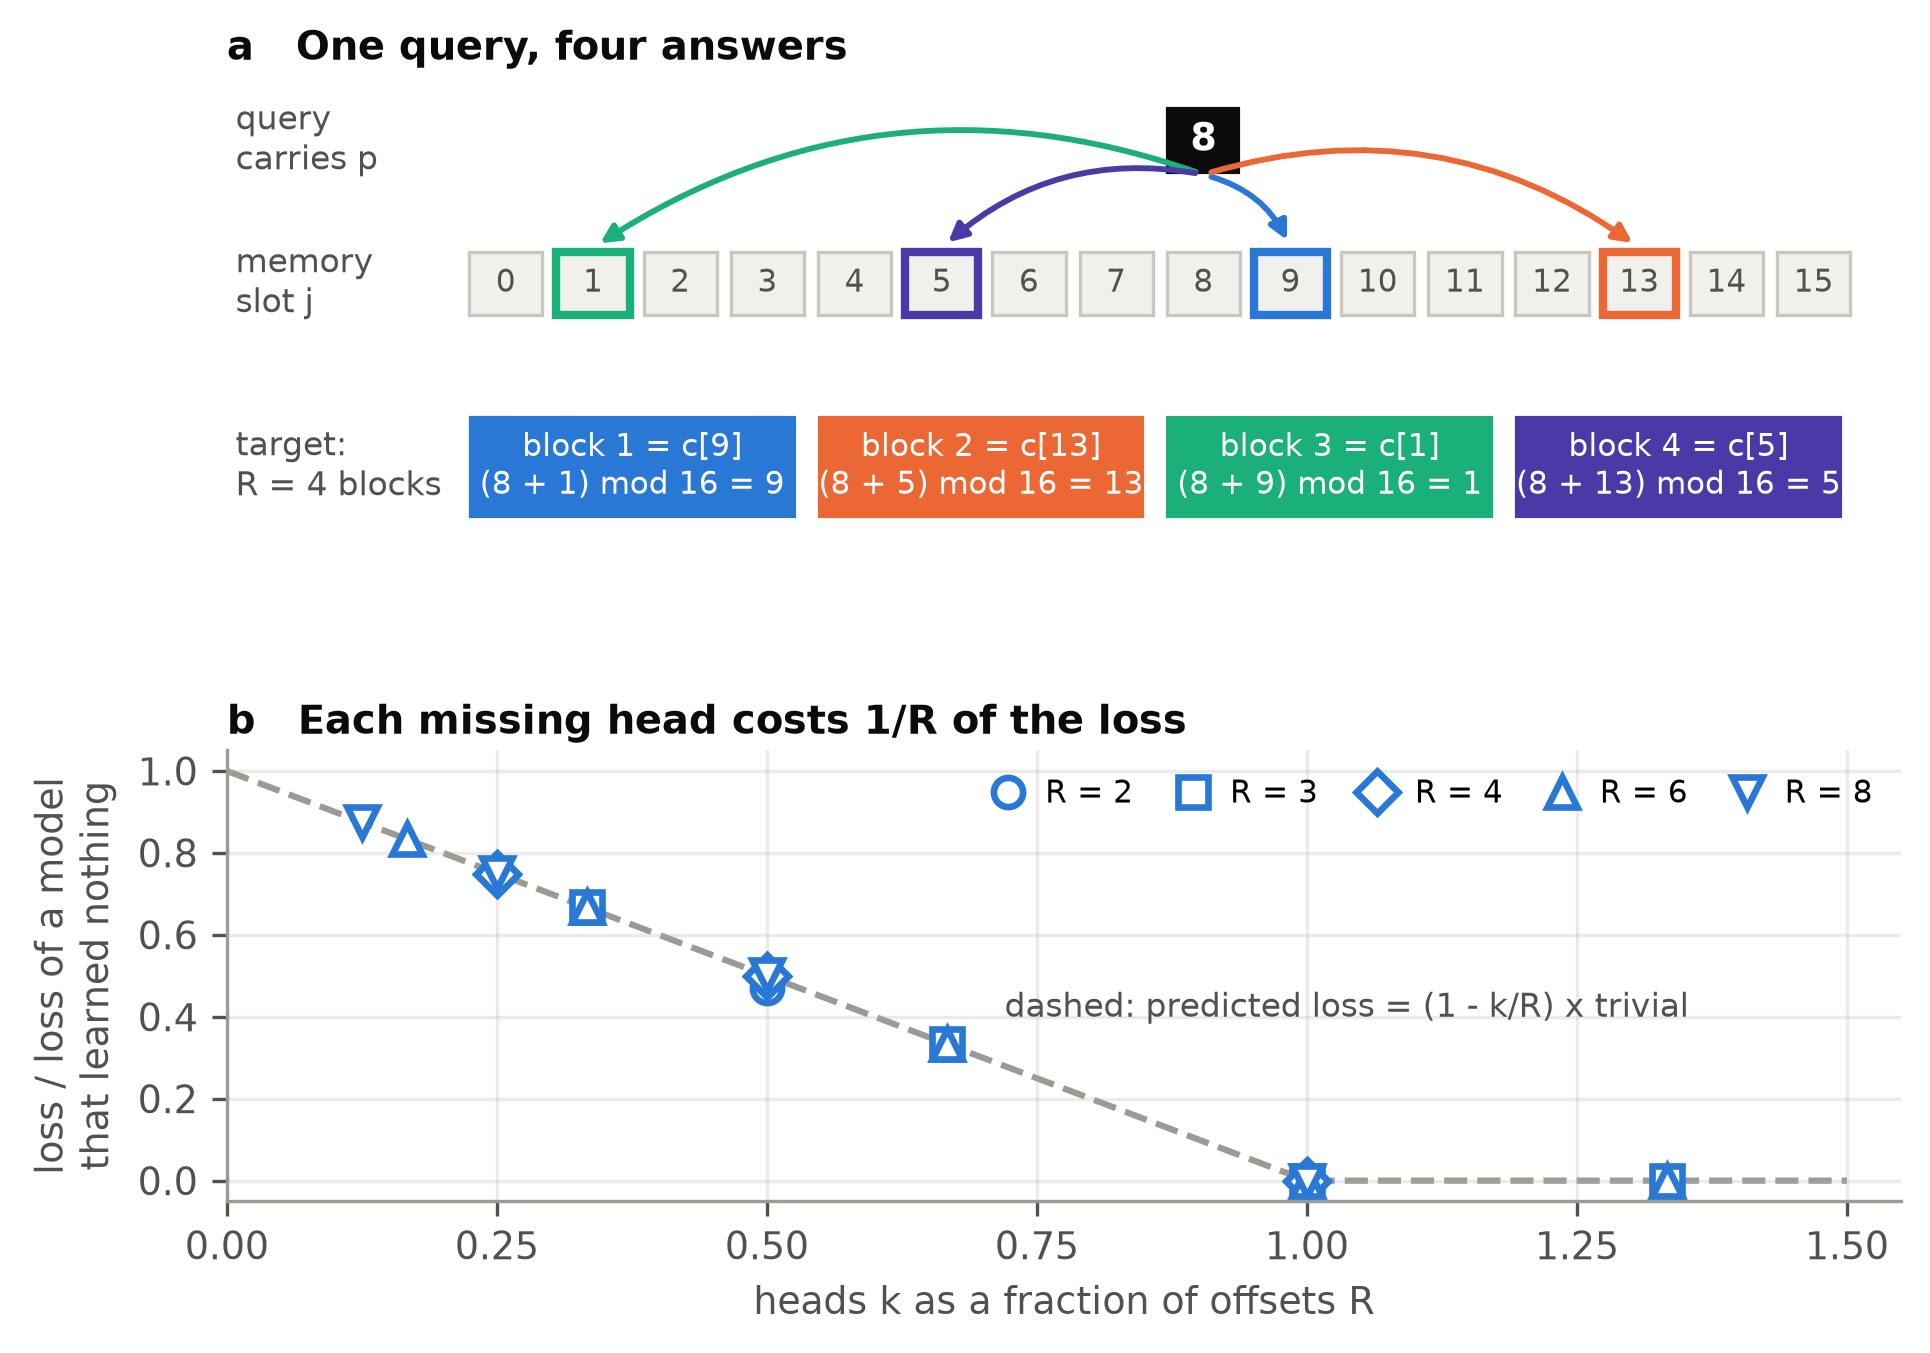
\includegraphics[width=\textwidth]{thesis_fig1_task.png}
  \caption{\textbf{The task.} (a) A query carrying position $p = 8$ must return the
  contents at four fixed offsets, $(8 + \delta) \bmod 16$ for $\delta = 1, 5, 9, 13$.
  (b) Dense models trained from scratch with $k$ heads, for tasks with
  $R = 2, 3, 4, 6, 8$ offsets. The loss, divided by the loss of a model that learned
  nothing, falls on the predicted line $1 - k/R$ and reaches zero at $k = R$. Every point
  is a measured training run.}
  \label{fig:task}
\end{figure}

\subsection{The task in matrices}

Collect the contents into one matrix, $C = [\,c_0\;c_1\;\cdots\;c_{N-1}\,] \in
\mathbb{R}^{m \times N}$, and write $e_p$ for the one-hot vector of position $p$. Reading
slot $p$ is then a matrix product, $c_p = C e_p$. Reading slot $p + \delta$ needs one more
matrix: the shift $P$, which moves every position forward by one, $P e_j = e_{j+1}$.
Shifting $\delta$ times is $P^\delta$, so
\begin{equation}
  c_{p+\delta} \;=\; C\,P^{\delta} e_p ,
  \qquad
  \text{target} \;=\;
  \begin{bmatrix} C P^{\delta_1} \\ \vdots \\ C P^{\delta_R} \end{bmatrix} e_p
  \;\in\; \mathbb{R}^{Rm}.
  \label{eq:targetmat}
\end{equation}
The task is a fixed linear map applied to the query's position. The model does not know
$C$, which is new for every sequence, so it has to find each $c_{p+\delta}$ by looking it
up. That is what attention does.

\subsection{What one head can do}

A head turns the query into a set of weights over the memory slots, and returns a weighted
average of what the slots hold. For a query $x$ and memory $Y$,
\begin{equation}
  q = W_Q x, \qquad K = W_K Y, \qquad
  a = \operatorname{softmax}\!\Bigl(\tfrac{K^\top q}{\sqrt{d_k}}\Bigr) \in \mathbb{R}^N, \qquad
  o = W_V Y a .
  \label{eq:head}
\end{equation}
The weights $a$ are non-negative and sum to one. The score for slot $j$ comes from
comparing the query's position code with the slot's position code, which is one entry of
the matrix $M = W_Q^\top W_K$:
\begin{equation}
  \text{score}(p, j) \;=\; e_p^\top M\, e_j = M_{pj}.
\end{equation}
To look from $p$ to $p + \delta$ for every $p$, the head needs large entries of $M$ at
positions $(p, p+\delta)$: a shifted diagonal. Figure~\ref{fig:heads}a shows these
diagonals, measured in a trained 4-head model, as stripes.

\begin{figure}[t]
  \centering
  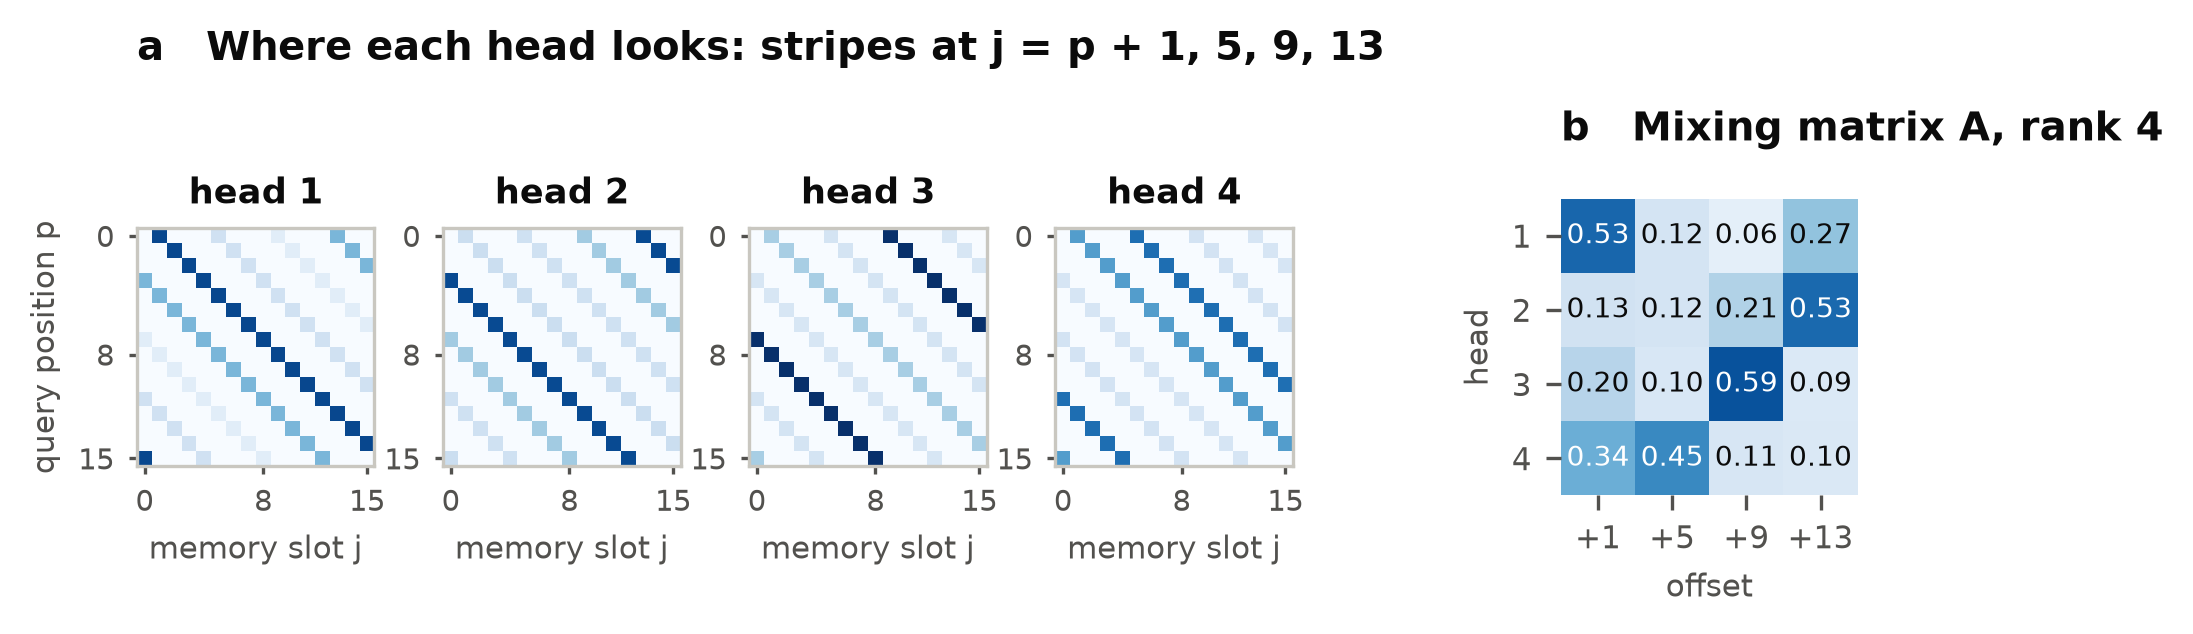
\includegraphics[width=\textwidth]{thesis_fig2_heads.png}
  \caption{\textbf{What the heads of a trained 4-head model do.} (a) Average attention
  from a query carrying position $p$ (rows) to memory slot $j$ (columns). Every head puts
  its weight on the four stripes $j = p + 1, 5, 9, 13$, so each head looks at all four
  offsets at once, in different proportions. (b) The mixing matrix $A$: the weight each
  head puts on each offset, averaged over queries. Each row sums to at least
  \thMixOnTarget{}. The matrix has full rank \thMixRank{}, which is what the task needs
  (Section~\ref{sec:rank}). Measured on a model trained for this figure, final loss
  $\thDenseFourLoss$.}
  \label{fig:heads}
\end{figure}

\subsection{Why the task needs exactly $R$ heads}
\label{sec:rank}

One might expect each head to specialise in one offset. The trained model shows otherwise:
every head looks at all four offsets, in different proportions (Figure~\ref{fig:heads}).
The reason the task still needs $R$ heads is a counting argument about these proportions.

Write $A_{hr}$ for the weight head $h$ puts on offset $\delta_r$. Since almost all of the
weight lands on the $R$ target slots, head $h$ returns (through $W_V$) one blend of the
$R$ contents it needs:
\begin{equation}
  u_h \;=\; \sum_{r=1}^{R} A_{hr}\, c_{p+\delta_r}.
\end{equation}
Stack the $R$ needed contents as the rows of a matrix $\widehat C \in \mathbb{R}^{R \times
m}$. Then $k$ heads together give the model $k$ blends,
\begin{equation}
  U \;=\; A\,\widehat C, \qquad A \in \mathbb{R}^{k \times R}.
  \label{eq:blend}
\end{equation}
The output layer is linear, so the best the model can do is multiply $U$ by some matrix
$B$. It needs $BA\widehat C = \widehat C$ for every possible content, which means
$BA = I_R$. That is possible only if $A$ has rank $R$, and a $k \times R$ matrix has rank
at most $k$. So
\begin{equation}
  \boxed{\;k \;\ge\; R\;}
\end{equation}
In words: \emph{each head gives one blend, and you cannot solve for $R$ unknowns from fewer
than $R$ blends.} Heads are free to blend offsets, as the trained heads do; what matters is
that the blends are independent. The measured $4 \times 4$ matrix in
Figure~\ref{fig:heads}b has rank \thMixRank{}, with smallest singular value \thMixMin{},
so it is safely invertible.

\paragraph{By hand, $R = 2$ and one head.} One head with weights $(\tfrac12, \tfrac12)$
returns $u = \tfrac12(c_1 + c_2)$. Knowing only $u$, the best guess for $c_1$ is $u$
itself, and so is the best guess for $c_2$. The error in each guess is
$\tfrac12(c_1 - c_2)$, whose variance is $\tfrac12$ when the contents have unit variance.
So one head leaves half of the loss of a model that learned nothing.

\paragraph{How much loss $k < R$ heads leave.} The same reasoning gives the whole curve.
With independent unit-variance contents, the best linear guess of $\widehat C$ from $U$ is
$\Pi\,\widehat C$, where $\Pi = A^\top (A A^\top)^{-1} A$ is the projection onto the rows
of $A$. The part left unexplained is $(I - \Pi)\widehat C$, and the trace of a projection
equals its rank, so the error is $R - k$ blocks out of $R$:
\begin{equation}
  L(k) \;=\; \Bigl(1 - \frac{k}{R}\Bigr) \Ltriv \qquad (k \le R),
  \label{eq:stair}
\end{equation}
where $\Ltriv$ is the loss of a model that always predicts the mean. Each missing head
costs $1/R$ of that loss. At $R = 4$ the measured losses with 1 and 2 heads are
\thLossOne{} and \thLossTwo{}, against predictions of \thPredOne{} and \thPredTwo{} from
$\Ltriv = \thTriv$. With 4 heads the loss is $\thLossFour$. Figure~\ref{fig:task}b shows
every task size at once. All points fall on the line, with the largest miss
\thStairMaxErr{} (in units of $\Ltriv$).

\paragraph{When is the task ``solved''?} A model is solved when its loss is within 2\% of
the gap between the dense model and the trivial one:
$L \le L_{\mathrm{dense}} + 0.02\,(\Ltriv - L_{\mathrm{dense}}) \approx 0.02$. By
Equation~\eqref{eq:stair} a model with $R - 1$ heads sits at $\Ltriv / R \ge 0.12$, far
above this bar, and a model with $R$ heads sits far below it. So the smallest solved model
has exactly $\kstar = R$ heads, with a wide margin on each side.

\subsection{Naming a head's job}

Because the offsets are known, a head can be given a name. A head's \emph{role} is the
offset where its average attention peaks, counted only if the peak is above $2/N$, twice
uniform. \emph{Role coverage} is the fraction of the true offsets that are the role of
some kept head. Figure~\ref{fig:heads} shows why this is a coarse label: a head that
blends all four offsets still gets only one name. Role coverage below 1 therefore does not
mean the circuit is wrong. The count $\kstar$ is exact; the naming is approximate.

%=========================================================================================
\section{A fixed supply shared by the heads}
\label{sec:supply}

\subsection{The supply as a diagonal matrix}

Give each head $h$ a supply $g_h \ge 0$ that multiplies its output, and fix the total:
\begin{equation}
  y \;=\; \sum_{h=1}^{H} g_h\, W_O^{(h)} o_h ,
  \qquad
  \sum_{h=1}^{H} g_h \;=\; H .
  \label{eq:supply}
\end{equation}
Here $W_O^{(h)}$ is the block of the output matrix that reads head $h$. In matrix form,
with $G = \operatorname{diag}(g)$, the layer is $y = W_O (G \otimes I_{d_k})\, o$ and the
constraint is $\operatorname{tr} G = H$. The ordinary dense layer is $G = I$, every head
at supply 1.

Every rule in this chapter feeds a set $S$ of $B$ heads equally, and starves the rest:
\begin{equation}
  g_h = \frac{H}{B} \;\text{ for } h \in S, \qquad g_h = 0 \;\text{ otherwise}.
  \label{eq:equal}
\end{equation}
The total is $B \cdot H/B = H$, as required. $B$ is never given to the model; each rule
arrives at it on its own.

\subsection{A starved head is removed exactly}

Put Equation~\eqref{eq:equal} into Equation~\eqref{eq:supply}. The starved heads are
multiplied by zero, and what remains is
\begin{equation}
  y \;=\; \sum_{h \in S} \Bigl(\tfrac{H}{B}\, W_O^{(h)}\Bigr) o_h ,
\end{equation}
which is an ordinary $B$-head layer whose output weights are scaled by $H/B$. Nothing is
approximated. A starved head also receives no gradient, because every path from its
weights to the loss passes through the factor $g_h = 0$.

\paragraph{By hand.} Take $H = 4$ heads that output one number each, $o = (3, 7, -1, 5)$,
with all output weights 1. Feed heads 1 and 3, so $g = (2, 0, 2, 0)$, which sums to 4.
The supplied layer gives $2\cdot 3 + 2\cdot(-1) = 4$. An ordinary 2-head layer with heads
1 and 3 and output weights 2 gives the same $4$. The dense layer would give $14$.

This matters for two reasons. For interpretation, the kept heads are the whole circuit,
with nothing hiding in the starved ones. For cost, a starved head does not need to be
computed at all, so a training step with $B$ heads switched on costs $B/H$ of a dense step.
The compute of a run is
\begin{equation}
  \text{compute} \;=\; \frac{1}{T} \sum_{t=1}^{T} \frac{B_t}{H}
  \;\;+\;\; \text{cost of any extra measurements},
  \label{eq:compute}
\end{equation}
where $T$ is the number of training steps; 1 means one dense run. This counts operations.
The current code still computes starved heads and multiplies them by zero, so these are
not wall-clock times.

\begin{figure}[t]
  \centering
  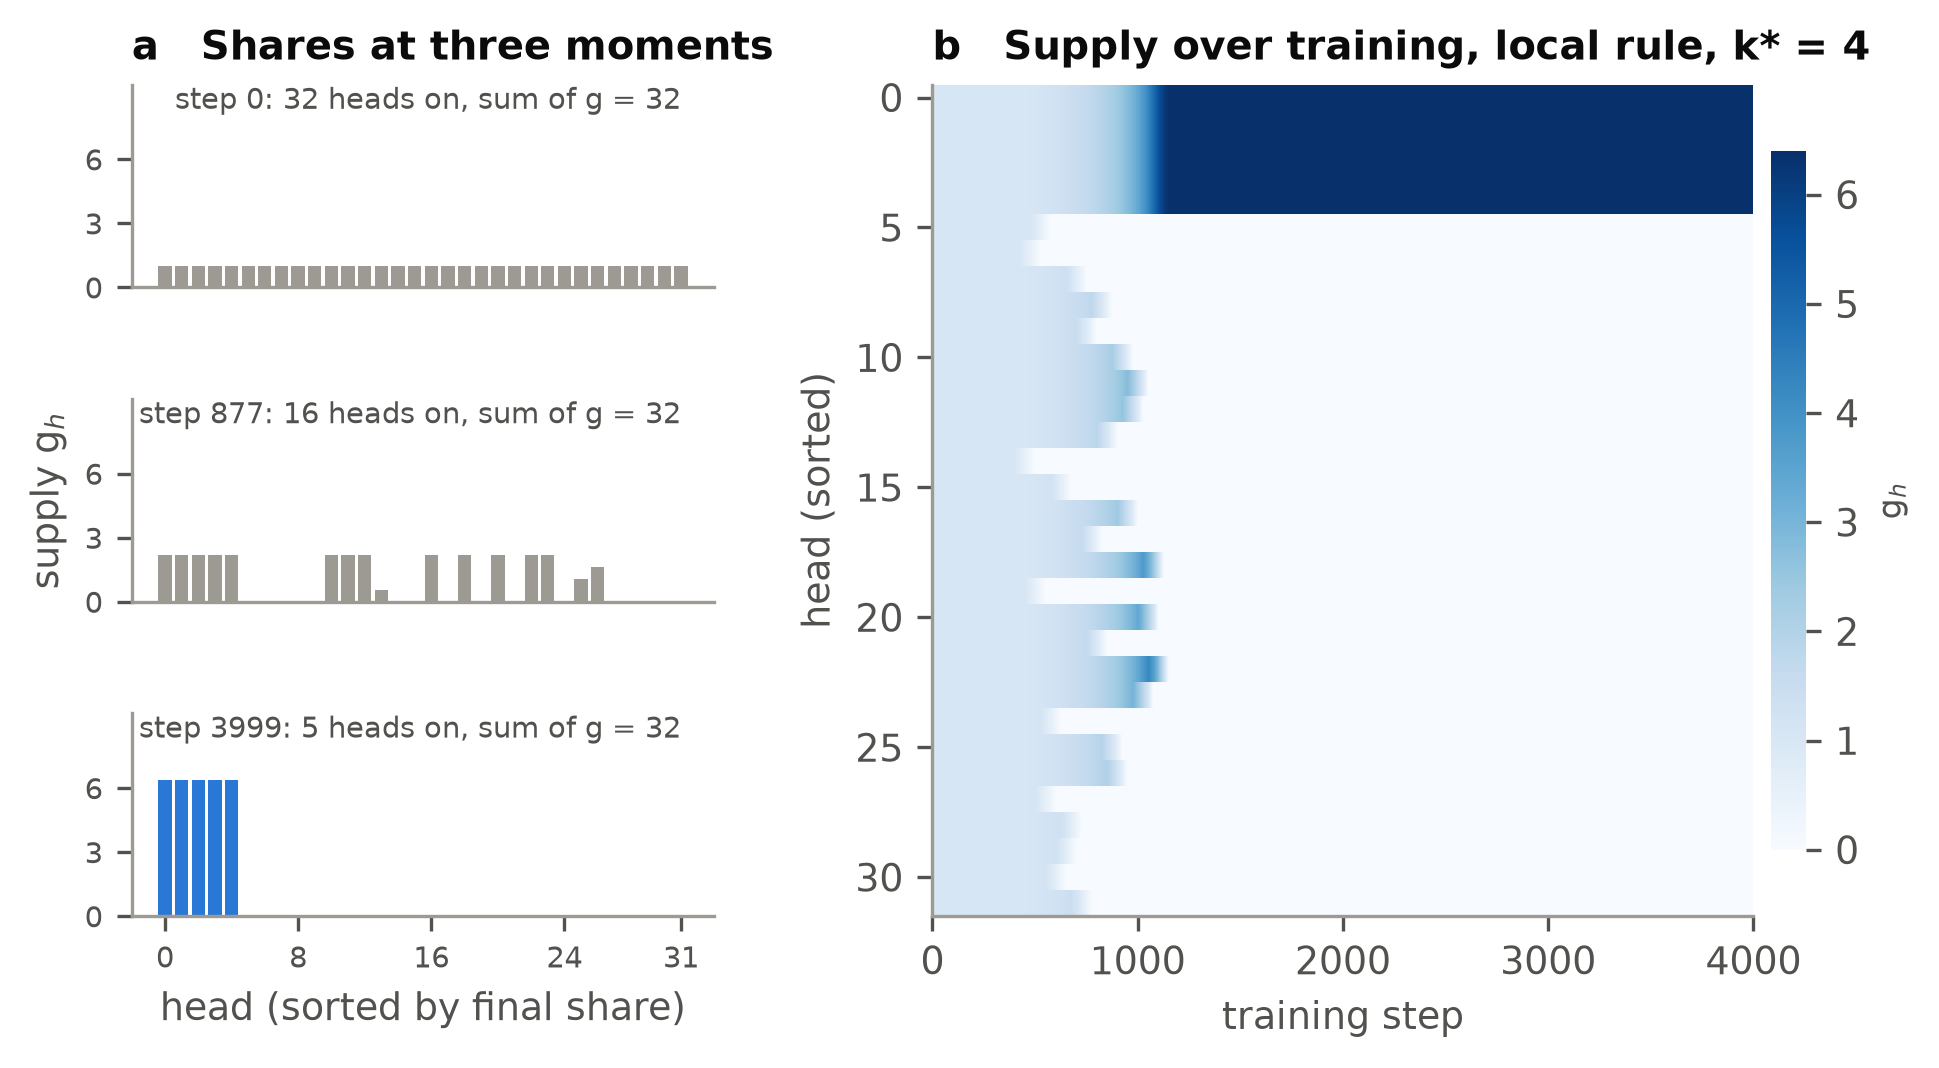
\includegraphics[width=\textwidth]{thesis_fig3_supply.png}
  \caption{\textbf{The supply during one real run} (local rule, Section~\ref{sec:local},
  task needs 4 heads). (a) The supply to every head at the start, midway through removal,
  and at the end. The shares change, but they always sum to 32. At the end
  \thFinalOn{} heads share the total, \thFinalShare{} each. (b) The same run over all
  training steps. Heads fade out gradually between roughly steps 400 and 1100, and the
  survivors grow brighter as they take over the freed supply.}
  \label{fig:supply}
\end{figure}

%=========================================================================================
\section{Rules for deciding who gets fed}
\label{sec:rules}

Every rule starts with all heads fed while the model first learns the task. After that it
moves the supply. The rules differ only in what they look at.

\subsection{The fixed threshold, and why it cannot count}
\label{sec:threshold}

Each head has a \emph{demand} $d_h$: how much it writes to the output, averaged over recent
steps. Standardise the demands, $z_h = (d_h - \bar d)/\sigma_d$, and feed every head that
stands out by more than $\kappa$ standard deviations:
\begin{equation}
  S = \{\, h : z_h > \kappa \,\}.
\end{equation}

\paragraph{By hand.} Eight heads with demands $d = (1,1,1,1,1,1,5,5)$. The mean is 2 and
the standard deviation 1.85. With $\kappa = 1$ the cut is $3.85$, so the last two heads
are fed: $B = 2$. Now make every demand ten times larger and add 100, $d' = 10d + 100$.
The mean becomes 120, the standard deviation 18.5, the cut 138.5, and the same two heads
are fed.

Standardising removes the scale and the level of the demands. What is left is only
\emph{how many heads stand out, and by how much}, which is a property of the shape of the
demand distribution. So $B$ equals the number of $z_h$ above $\kappa$, whatever the task
needs. Nothing in the rule can see $\kstar$. Figure~\ref{fig:count}b checks this on every
fixed-threshold run: counting the standardised demands above $\kappa$ predicts the number
of heads kept in \thThrMatch{} runs.

\subsection{A feedback loop on the loss}
\label{sec:loop}

The repair is to let the threshold move, driven by how far the loss $\widehat L_t$ is from
a target $L^\star$ (2\% of $\Ltriv$, the solved bar):
\begin{equation}
  \kappa_{t+1} \;=\; \kappa_t + \eta\,\bigl(\ln L^\star - \ln \widehat L_t\bigr),
  \qquad \eta = 0.003 .
\end{equation}
If the loss is too high, $\kappa$ falls, the cut drops and more heads are fed. If the loss
is below target, $\kappa$ rises and heads are starved. It works like a thermostat.

\paragraph{By hand, where it settles.} Use the staircase from Equation~\eqref{eq:stair} at
$R = 4$: $L(1) \approx 0.75$, $L(2) \approx 0.50$, $L(3) \approx 0.25$, and almost 0 from 4
heads up. With target $0.02$, start at 6 heads and remove one head whenever the loss is
below target, add one otherwise: $6 \to 5 \to 4 \to 3$. At 3 heads the loss is $0.25$,
above target, so add one: $3 \to 4$. At 4 the loss is below target again, so the loop
tries 3, and so on. It settles at the smallest $B$ that meets the target,
\begin{equation}
  B^\star \;=\; \min\{\, B : L(B) \le L^\star \,\} \;=\; \kstar ,
\end{equation}
and this holds for any target between $L(\kstar)$ and $L(\kstar - 1)$, a range of several
orders of magnitude here. The walk also shows the loop's weakness: it keeps testing one
head fewer, so it flips between $\kstar$ and $\kstar - 1$.

\subsection{The stall gate}

Early in training the loss is high for every $B$, because the model has not learned yet,
so the loop above feeds every head and may never recover. The fix is to wait before
feeding more heads while the loss is still falling. Let $\bar L_t$ be a slower average of
the loss, and $\rho_t = (\bar L_t - \widehat L_t)/\bar L_t$ how fast it is still falling.
\begin{itemize}
\item Loss above target \emph{and} still falling ($\rho_t > \varepsilon$): wait.
\item Otherwise: update $\kappa$ as before. Starving heads is never delayed.
\end{itemize}
With $\varepsilon = 0.02$: slow average $0.030$ and current loss $0.024$ give
$\rho = 0.20$, so the gate waits; slow average $0.0244$ and current $0.0240$ give
$\rho = 0.016$, so the loop feeds.

\subsection{The pruning baseline}

The standard alternative is iterative pruning with gradient importance \cite{michel2019},
run during training on the same schedule. Every 25 steps the open head with the smallest
$|\partial L / \partial m_h|$ is removed, where $m_h$ is a 0/1 mask on head $h$. Pruning
stops once the loss stays above the same solved bar for four checks in a row, and the
last head removed is put back. There is no fixed total: a removed head's share goes to
nobody.

\subsection{The local rule: each head earns its share}
\label{sec:local}

The last rule has no loss target. Every 25 steps it asks, for each head, what \emph{no
other head can provide}. Collect the head outputs on a fresh batch into a matrix
$Z = [\,Z_1\;\cdots\;Z_H\,]$ (one row per token) and the targets into $T$. For a set of
open heads $S$, the best linear read-out and its error are
\begin{equation}
  W_S = (Z_S^\top Z_S)^{-1} Z_S^\top T, \qquad
  E(S) = \lVert T - Z_S W_S \rVert^2 .
\end{equation}
The value of an open head is how much the error rises when it is removed and the others
refit their read-out; the value of a starved head is how much the error falls if it is
fed:
\begin{equation}
  v_h = E(S \setminus \{h\}) - E(S) \quad (h \text{ open}), \qquad
  v_h = E(S) - E(S \cup \{h\}) \quad (h \text{ starved}).
\end{equation}
The rule closes the cheapest open head if $v_h$ is below a price $\pi = 0.03\,\Ltriv$, or
reopens the most valuable starved head if $v_h > 2\pi$. The factor of two stops a head at
the price from flickering. One change is made per check.

\paragraph{By hand: a copy is worth nothing.} Heads A and B both output the same signal
$z$; head C outputs $w$; the target is $z + w$. Remove A and B still carries $z$, so after
refitting nothing is lost: $v_A = 0$. Likewise $v_B = 0$. Remove C and nobody carries $w$:
$v_C = \operatorname{var}(w)$. So one of the copies is closed first. Once it is gone, the
other is no longer a copy, its value jumps, and it stays. A head's value depends on what
the other heads do, which per-head importance scores cannot capture.

Two additions make the rule work in practice. \emph{Fade}: a closing head's supply falls
over 100 steps instead of at once, with the total kept at $H$ throughout
(Figure~\ref{fig:supply}b). \emph{Early start}: supply begins to move at step 400 (10\%
of training) instead of step 1000. The checks are charged in Equation~\eqref{eq:compute}:
each uses 512 fresh sequences through the forward pass, which costs $4/3$ of a dense
training step.

%=========================================================================================
\section{Results}
\label{sec:results}

All runs use $H = 32$ heads, $N = 16$ slots, $d_k = 32$ and 4000 training steps, with
$\kstar \in \{2, 3, 4, 6, 8\}$. The number of heads kept, $B$, is the median over the last
part of training, after the supply has settled. A run \emph{fails} if its final loss is
above the solved bar. The chapter draws on \thNRuns{} runs in total.

\subsection{Counting heads}

\begin{figure}[t]
  \centering
  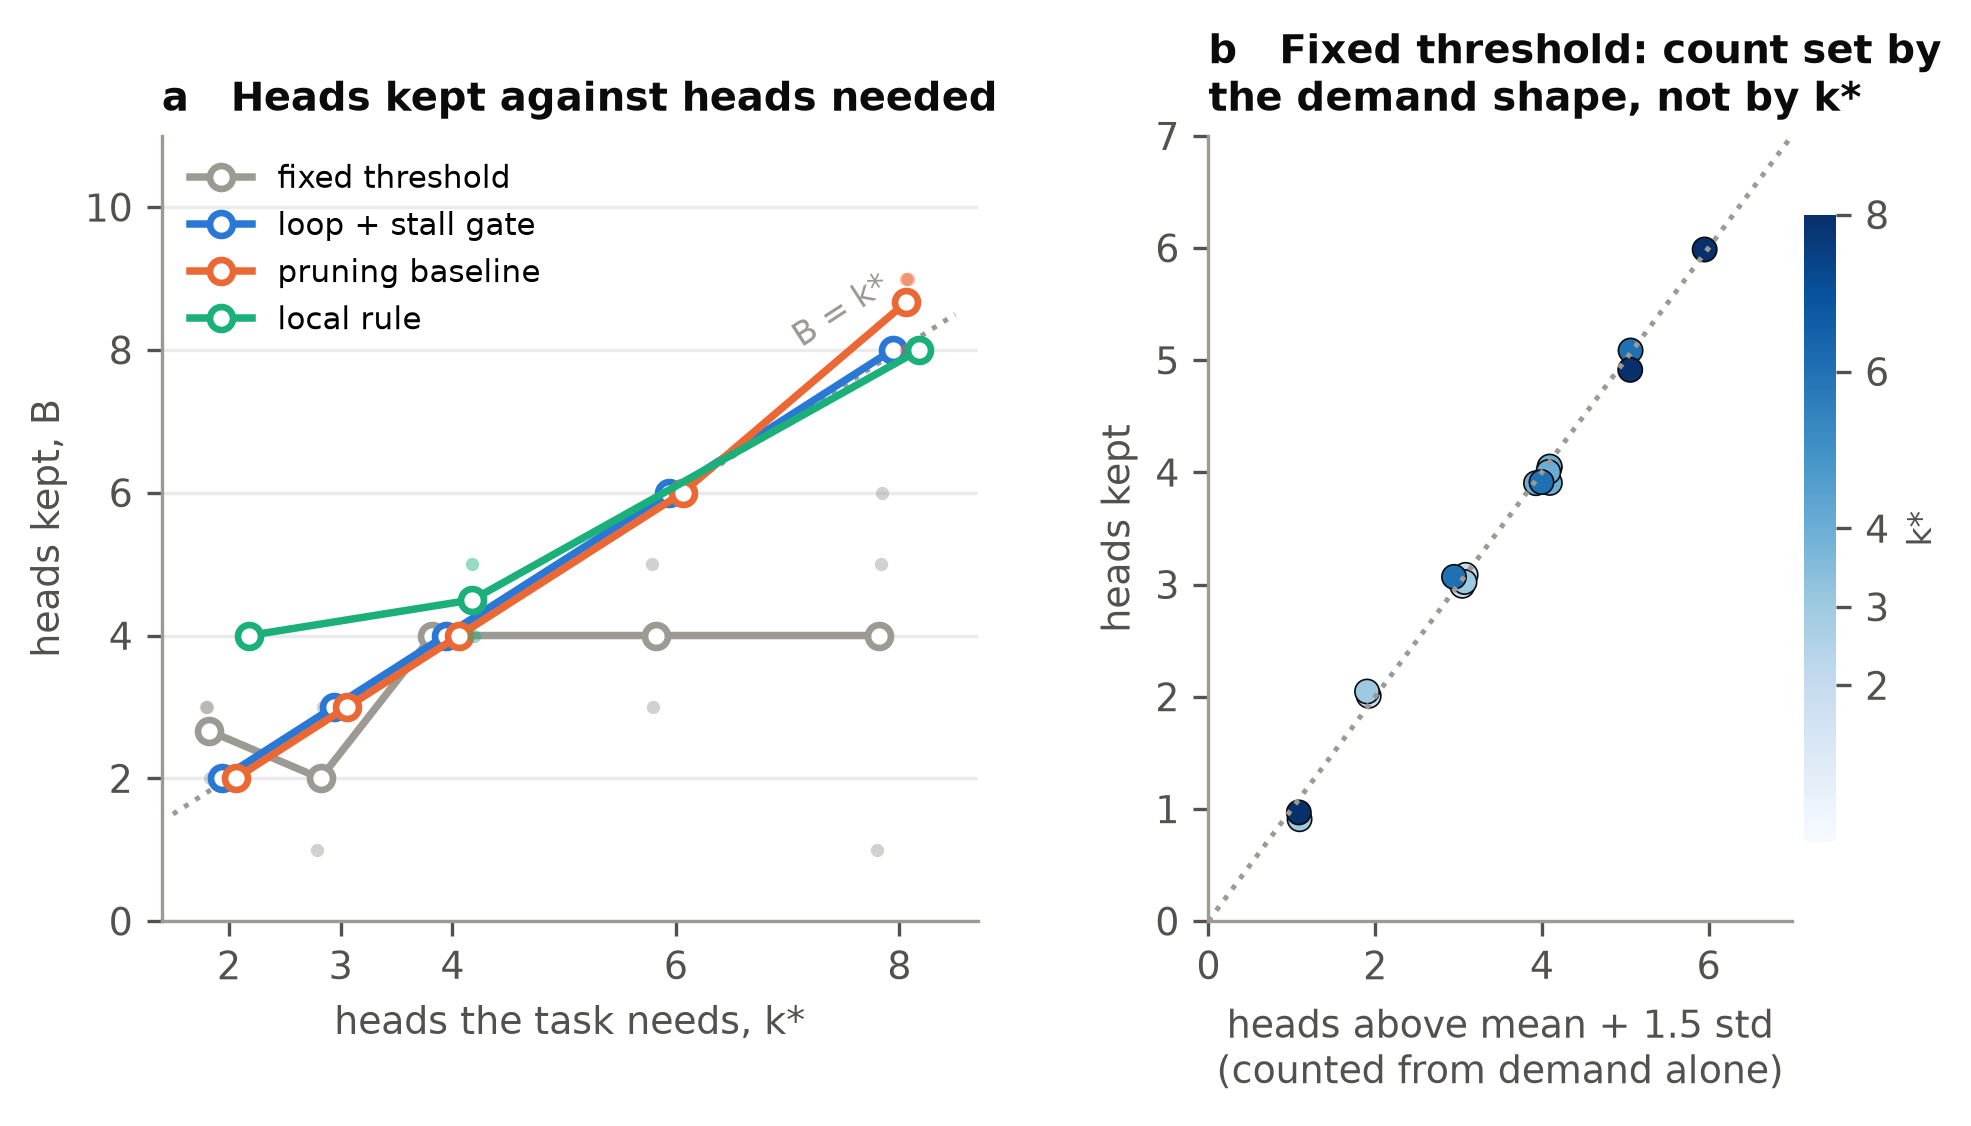
\includegraphics[width=\textwidth]{thesis_fig4_count.png}
  \caption{\textbf{Heads kept against heads needed.} (a) Open circles are the mean over
  seeds, small dots single runs; the dotted line is $B = \kstar$. The fixed threshold
  (grey) flattens at about 4 heads. The loop with stall gate and the pruning baseline lie
  on the line. The local rule is right at 8 but keeps too many heads at 2.
  (b) For every fixed-threshold run, the number of standardised demands above
  $\kappa = 1.5$ (horizontal) predicts the number of heads kept (vertical) exactly. Colour
  is $\kstar$: runs for very different tasks sit at the same count.}
  \label{fig:count}
\end{figure}

\begin{table}[t]
  \centering\small
  % generated by experiments/thesis_figures.py, do not edit
\begin{tabular}{l ccccc c c c}
\toprule
& \multicolumn{5}{c}{heads kept $B$ when the task needs $k^\star$} & & & \\
\cmidrule(lr){2-6}
rule & 2 & 3 & 4 & 6 & 8 & miss (heads) & failed runs & compute \\
\midrule
fixed threshold & 2.7 & 2.0 & 4.0 & 4.0 & 4.0 & 1.53 & 8/17 & 0.60 \\
feedback loop & 2.0 & 3.0 & 4.0 & 6.0 & 8.0 & 0.00 & 11/49 & 0.41 \\
loop + stall gate & 2.0 & 3.0 & 4.0 & 6.0 & 8.0 & 0.00 & 13/50 & 0.42 \\
pruning baseline & 2.0 & 3.0 & 4.0 & 6.0 & 8.7 & 0.13 & 0/15 & 0.43 \\
pruning, told $k^\star$ & 2.0 & 3.0 & 4.0 & 6.0 & 8.0 & 0.00 & 0/15 & 0.43 \\
local rule & 4.0 & -- & 4.5 & -- & 8.0 & 0.83 & 0/6 & 0.39 \\
\bottomrule
\end{tabular}

  \caption{\textbf{Every rule on every task size.} ``Miss'' is the average of
  $|B - \kstar|$. ``Failed runs'' counts runs whose final loss is above the solved bar.
  ``Compute'' is Equation~\eqref{eq:compute}, where 1 is one dense training run. Dashes
  are task sizes not run for that rule.}
  \label{tab:count}
\end{table}

Table~\ref{tab:count} and Figure~\ref{fig:count} give the main comparison.

\begin{itemize}
\item \textbf{The fixed threshold does not count.} It keeps 4 heads whether the task
      needs 4, 6 or 8, and misses by \thThrErr{} heads on average. The fitted slope of
      $B$ against $\kstar$ is \thThrSlope{}, where 1 would mean it tracks the task.
      Section~\ref{sec:threshold} explains why.
\item \textbf{The feedback loop counts exactly}, with and without the stall gate: $B =
      \kstar$ at all five sizes, miss \thLoopErr{}. But it flips between $\kstar$ and
      $\kstar - 1$, and a model one head short fails the task, so \thLoopBad{} runs of
      the plain loop and \thGateBad{} with the gate end above the bar.
\item \textbf{Pruning with the same bar counts as well} (miss \thPruneErr{}) and never
      fails (\thPruneBad{}), because it stops for good instead of flipping. Finding the
      count comes from checking the loss against a bar, not from the fixed total.
\item \textbf{The local rule} is right at $\kstar = 8$ but keeps \thLocalTwo{} heads
      where 2 are needed. It never fails (\thLocalBad{}).
\end{itemize}

\subsection{Is the loss target a tuned setting?}

\begin{figure}[t]
  \centering
  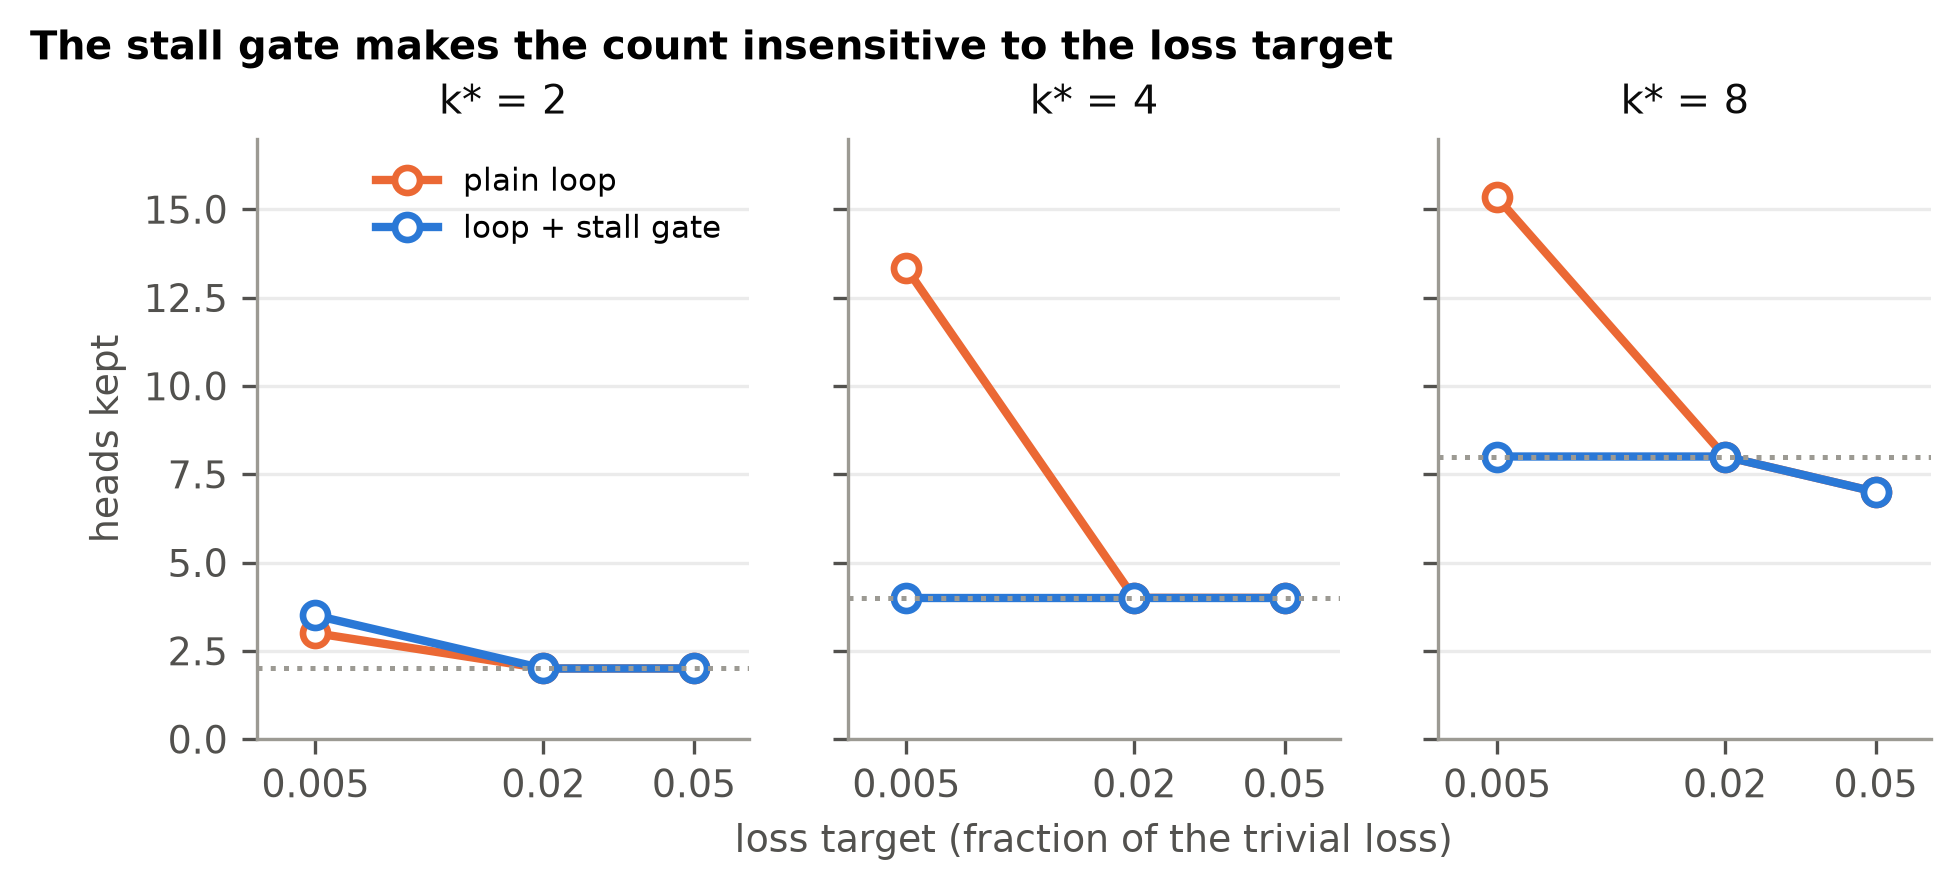
\includegraphics[width=\textwidth]{thesis_fig5_target.png}
  \caption{\textbf{Heads kept as the loss target changes tenfold.} The dotted line is the
  right answer. At the tightest target the plain loop (orange) feeds up to 15 heads,
  because it reacts to the high loss early in training. With the stall gate (blue) the
  count is exact at the default target and within two heads everywhere.}
  \label{fig:target}
\end{figure}

The loop needs a target. If it only works at one target, the target is a hidden setting.
Figure~\ref{fig:target} varies it tenfold. Averaged over the three targets and three task
sizes, the plain loop misses by \thTargetPlain{} heads and the loop with the stall gate by
\thTargetGate{}.

Two controls check the gate itself.
\begin{itemize}
\item \emph{Is the gate's own threshold $\varepsilon$ tuned?} Varying $\varepsilon$
      sixteenfold (0.005 to 0.08) leaves the count exact at every size; the largest miss
      is \thEpsErrMax{} heads.
\item \emph{Is the gate just a slower loop?} Running the plain loop ten times more slowly
      breaks it: it misses by \thSlowErr{} heads. The gate works because it waits for the
      right moment, not because it is slow.
\end{itemize}

\subsection{Compute, and the loss while heads are removed}

\begin{figure}[t]
  \centering
  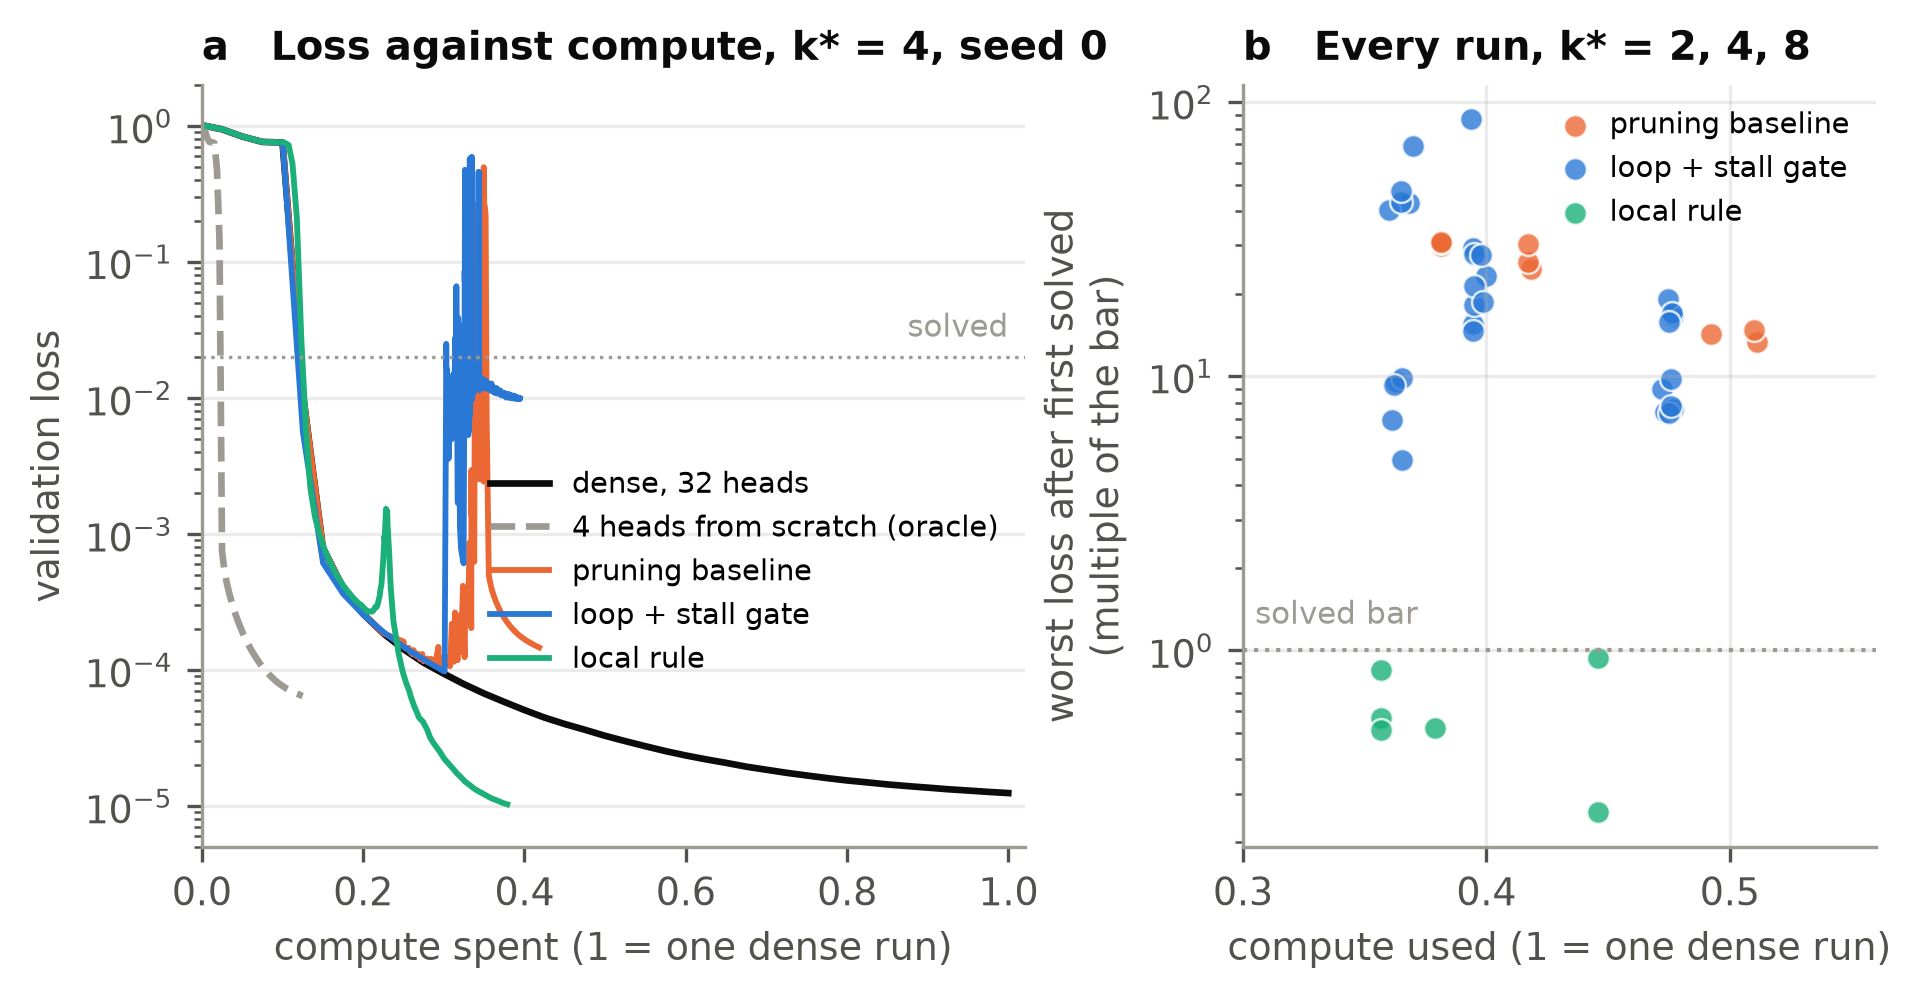
\includegraphics[width=\textwidth]{thesis_fig6_compute.png}
  \caption{\textbf{Compute and stability.} (a) Validation loss against compute spent, for
  one run of each rule on the 4-head task. The loop (blue) and pruning (orange) jump far
  above the solved bar when they remove heads; the local rule (green) rises briefly and
  stays below it, then keeps improving. The dense model (black) and a 4-head model trained
  from scratch (grey dashed, possible only if the answer is known) are shown for
  comparison. (b) Every run on the 2-, 4- and 8-head tasks: compute used against the
  worst loss after the run first reached the solved bar, as a multiple of the bar. Only
  the local rule stays below 1.}
  \label{fig:compute}
\end{figure}

Figure~\ref{fig:compute} compares the three rules that find a count. The median of the
worst loss after first reaching the solved bar is \thWorstGate{} times the bar for the
loop, \thWorstPrune{} for pruning, and \thWorstLocal{} for the local rule. Only the local
rule never goes back above the bar. The fade is what keeps it there, and the early start
is what saves compute: the local rule uses \thLocalCompute{} of a dense run, against
\thGateCompute{} for the loop and \thPruneCompute{} for pruning.

Compared with the dense model given the same compute, the local rule has the lower loss in
\thBelowSame{} runs. It matches what the dense model reaches after a \emph{full} run in
only \thBelowFull{}. So the fair statement is ``usually better than dense at equal
compute'', not ``as good as dense at a third of the cost''. The 4-head model trained from
scratch is cheaper still, so the saving is the saving from \emph{not knowing} $\kstar$ in
advance.

\subsection{What did not work}

These results are kept because each one rules something out.
\begin{itemize}
\item \textbf{Other rules that ignore the loss.} Cutting at the largest gap in the sorted
      demands, splitting the demands into two clusters, making flow grow with demand to a
      power, and giving groups of heads a shared supply: none tracks $\kstar$. The
      argument of Section~\ref{sec:threshold} applies to all of them, since none sees the
      loss.
\item \textbf{Groups of heads did not pack the circuit together.} The circuit spread over
      nearly every group, because each group kept at least one head by construction.
\item \textbf{A delay between demand and supply, and averaging demand across neighbours,}
      changed nothing over the ranges tried.
\item \textbf{Demand is not the best measure of a head's importance.} Its rank correlation
      with the damage done by removing a head is \thRhoDemand{}, against \thRhoQnorm{} for
      the size of the head's query and \thRhoEntropy{} for how sharply it attends.
\item \textbf{A second task.} On a task where heads are interchangeable and the number
      needed comes from capacity rather than function, the loop failed in every run
      (\thQsaBad{} failed). The method is shown on one task only.
\end{itemize}

%=========================================================================================
\section{What this shows, and what it does not}
\label{sec:claims}

\paragraph{What holds.}
\begin{enumerate}
\item \textbf{A task with a known circuit size.} A rank argument shows it needs exactly
      $R$ heads, predicts the loss of every smaller model, and the measurements agree.
      Heads can be named by their offsets, though trained heads blend offsets, so the
      names are approximate.
\item \textbf{Starving is removing.} A fixed total supply turns switching heads off into
      an exact reduction to a smaller layer, which is what makes the compute saving real
      in principle.
\item \textbf{Why the obvious rule fails.} A rule that looks only at how demands are
      spread cannot know how many heads the task needs. This is shown by the argument and
      confirmed run by run.
\item \textbf{Checking the loss finds the count.} The feedback loop gets it exactly at
      every size, and the stall gate makes it hold over a tenfold range of targets.
\item \textbf{Removing heads without losing the task.} The local rule with fade and early
      start is the only rule that never falls back above the solved bar, at the lowest
      compute of the three.
\end{enumerate}

\paragraph{What does not hold, or is not claimed.}
\begin{itemize}
\item \textbf{The count is not unique to the supply idea.} Pruning with the same bar
      finds it too, and fails less often than the loop.
\item \textbf{This is not discovery from first principles.} ``The fewest heads that reach a
      loss bar'' is close to the definition of the smallest circuit. The contribution is
      doing it in one training run rather than a sweep over sizes.
\item \textbf{The local rule keeps too many heads for small tasks}, and its price moves the
      count. It has been run on only two seeds per size.
\item \textbf{The method is shown on one synthetic task}, with one layer.
\end{itemize}

\paragraph{The experiments that would settle it.} In order of importance: (1) train
$\kstar$ heads from scratch for the same compute as the local rule; if that matches its
loss, the compute claim fails. (2) Run the local rule with free supply, no fixed total,
to test whether the total matters at all. (3) Ten seeds for the local rule. (4) Wall-clock
time with starved heads actually skipped. (5) A two-layer model, where heads in different
layers must cooperate.

\begin{thebibliography}{9}
\bibitem{michel2019} P.~Michel, O.~Levy, G.~Neubig.
  Are sixteen heads really better than one? \emph{NeurIPS}, 2019.
\bibitem{voita2019} E.~Voita, D.~Talbot, F.~Moiseev, R.~Sennrich, I.~Titov.
  Analyzing multi-head self-attention: specialized heads do the heavy lifting, the rest
  can be pruned. \emph{ACL}, 2019.
\end{thebibliography}

\end{document}
